\documentclass[11pt,a4paper,twocolumn]{article}
\usepackage[margin=1.8cm,columnsep=0.6cm]{geometry}
\usepackage{mathptmx}
\usepackage[T1]{fontenc}
\usepackage{graphicx,booktabs,cite,caption}
\usepackage[hidelinks]{hyperref}
\urlstyle{same}
\captionsetup{labelfont=bf,skip=3pt}
\setlength{\textfloatsep}{8pt}
\setlength{\floatsep}{6pt}
\renewcommand{\arraystretch}{1.05}
\makeatletter
\renewcommand\section{\@startsection{section}{1}{\z@}{-1.4ex plus -.4ex}{0.6ex}{\normalfont\large\bfseries}}
\makeatother

\title{\vspace{-1.2cm}\textbf{Predicting the Remaining Useful Life of Jet Engines with Linear Regression and Decision Trees}}
\author{CSC1181/CSC1203 Machine Learning Project \\ \small Code: \url{https://github.com/weeblul/rul-maintenence-Project-Stats}}
\date{\vspace{-0.9cm}}

\begin{document}
\twocolumn[
\maketitle
\begin{center}
{\small\textbf{Contribution and roles}}\par\vspace{2pt}
\begin{tabular}{lp{13.3cm}}
\toprule
\textbf{Member} & \textbf{Contribution} \\
\midrule
Daksh Jadhav & Model training (baseline, linear regression, decision tree depth tuning, logistic regression); evaluation, error analysis; report writing and integration \\
Abdul Gaffar Nagori & Data loading and RUL labels; EDA and sensor analysis; feature selection; preprocessing (RUL cap, rolling mean, scaling); engine-level train/validation split \\
Jamie & Mock ERP database (SQLite, six tables) and its access layer; stock, procurement and scheduler agents with cost-limit and deferral rules; audit-log explanations \\
Rajesh & Engine simulator and predictor; risk trigger (risk $\geq$ 0.7); Streamlit dashboard with fleet view, approval queue and KPIs; end-to-end testing \\
\bottomrule
\end{tabular}
\end{center}
\vspace{0.3cm}
]

\begin{abstract}
\noindent
We predict how many cycles a jet engine has left before it fails (its Remaining Useful Life, RUL) using NASA's C-MAPSS FD001 and FD003 data. With ten smoothed sensors, a decision tree reaches a test RMSE of 18.29 on FD001 and 19.95 on FD003, against 43.08 and 42.50 for a mean baseline and about 21 for linear regression. Logistic regression flags engines failing within 30 cycles with precision 0.81 and recall 0.61.
\end{abstract}

\section{Problem and Data}
An engine repaired too late may fail, and one repaired too early wastes parts. We set two targets: RUL in cycles (regression) and whether the engine fails within 30 cycles (classification). We measure RUL with RMSE and MAE, and the classifier with accuracy, precision, recall and F1.

C-MAPSS~\cite{saxena2008,nasadata} contains simulated engines that run until they fail. Each row is one cycle: engine number, cycle, three operating settings and 21 sensors. FD001 has one fault (HPC) and FD003 has two (HPC and fan). Each has 100 training and 100 test engines, giving 45,351 training rows and 29,692 test rows. Test engines stop before failure and NASA gives their true RUL. There are no missing values.

\section{Literature Review}
Saxena et al.~\cite{saxena2008} released C-MAPSS for the PHM08 challenge. Heimes~\cite{heimes2008} won it with a recurrent neural network and capped the RUL target while an engine is still healthy; we use the same idea with a cap of 125. Babu et al.~\cite{babu2016} used a convolutional neural network (CNN) and got RMSE 18.45 on FD001 and 19.82 on FD003. Zheng et al.~\cite{zheng2017} used an LSTM (16.14 and 16.18), and Li et al.~\cite{li2018} reached 12.61 and 12.64 with a deeper CNN. These models are complex; we test how close simpler ones get.

\section{Methods}
\textbf{Preprocessing.} Seven sensors (s1, s5, s6, s10, s16, s18, s19) barely change (standard deviation below 0.02), so we removed them. The RUL of a training row is the engine's last cycle minus the current cycle, capped at 125 because a healthy engine shows no wear yet. Each sensor was smoothed with a 5-cycle rolling mean per engine to reduce noise, then scaled to 0-1 with MinMaxScaler fitted on training data only.

\textbf{Feature selection.} We ranked the remaining 14 sensors by absolute correlation with RUL and added them in order, skipping any sensor correlated above 0.9 with one already chosen. This dropped s8 (close to s13) and s14 (close to s9) and left ten features: s11, s4, s17, s13, s3, s2, s9, s20, s21 and s15. Sensors s7, s12 and s15 correlate weakly overall because the two FD003 faults push them in opposite directions (Fig.~\ref{fig:sensors}).

\textbf{Models.} The baseline predicts the mean training RUL. Linear regression fits one weight per sensor. A decision tree regressor asks yes/no questions about the sensors, so it can learn non-linear patterns such as wear speeding up near the end of life. Logistic regression predicts the probability of failing within 30 cycles. All models come from scikit-learn~\cite{sklearn}.

\textbf{Validation.} Rows from the same engine are very similar, so we split by engine: 160 for training and 40 for validation. We tried tree depths from 2 to 15 (Fig.~\ref{fig:depth}). Training error kept falling, but validation error was lowest at depth 9 (RMSE 19.38) and then rose, a sign of overfitting. The final models were trained on all 200 engines and tested once on the official test sets, at the last cycle of each engine.

\begin{figure*}[t]
\centering
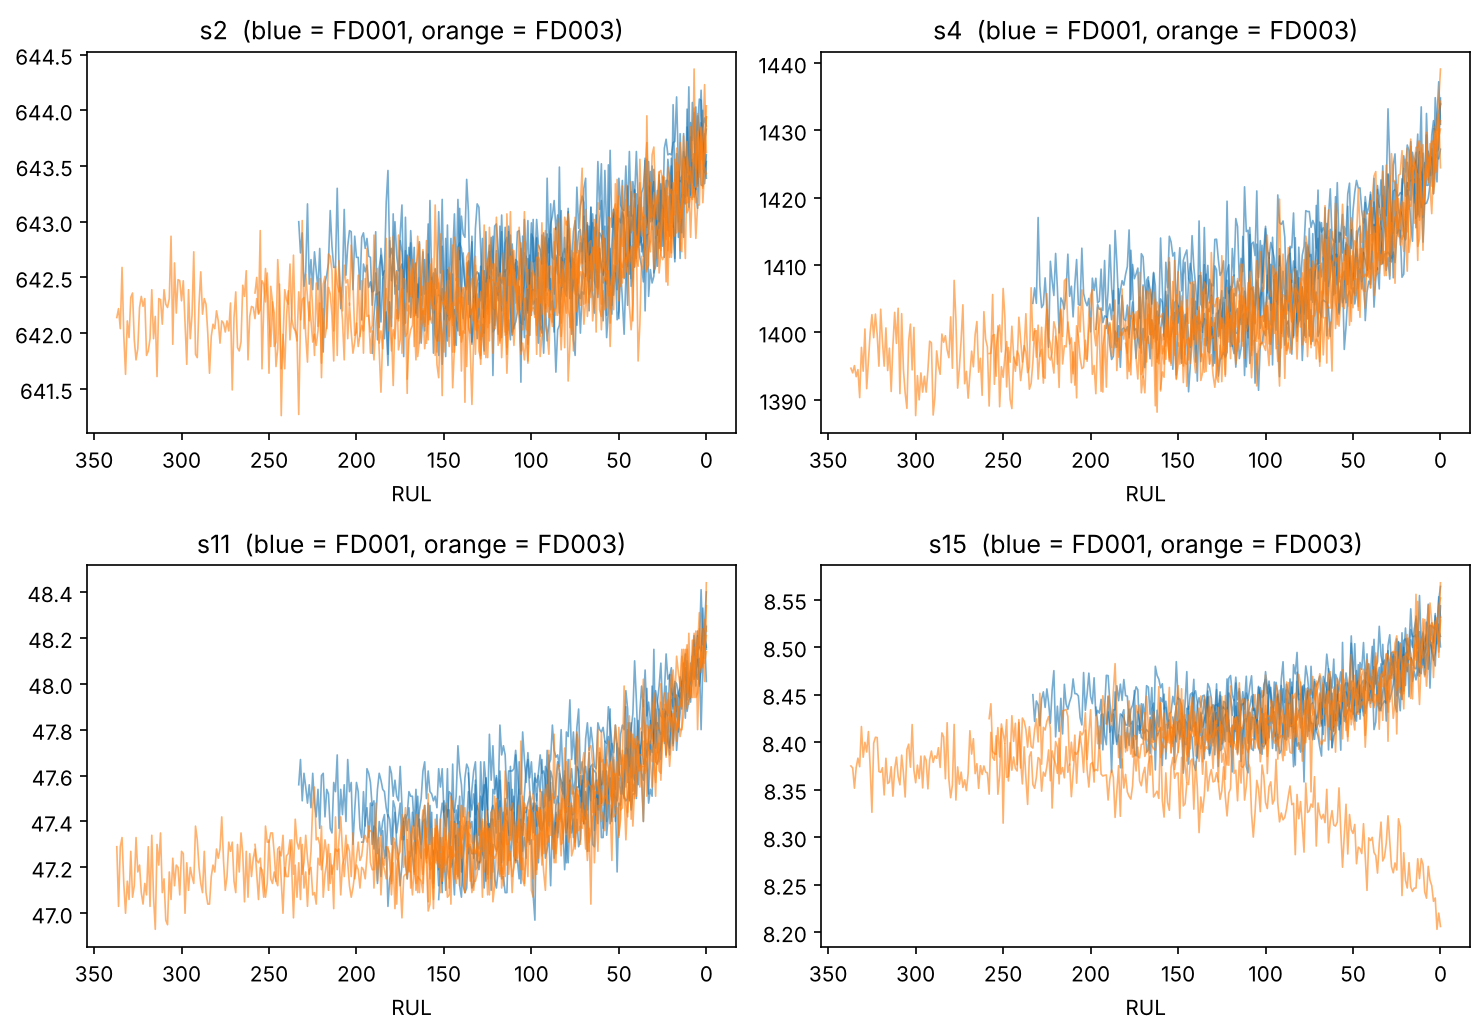
\includegraphics[width=0.8\textwidth]{sensors.png}
\caption{Four sensors for five FD001 (blue) and five FD003 (orange) engines as they approach failure (RUL = 0). s15 goes up for some FD003 engines and down for others.}
\label{fig:sensors}
\end{figure*}

\begin{figure}[t]
\centering
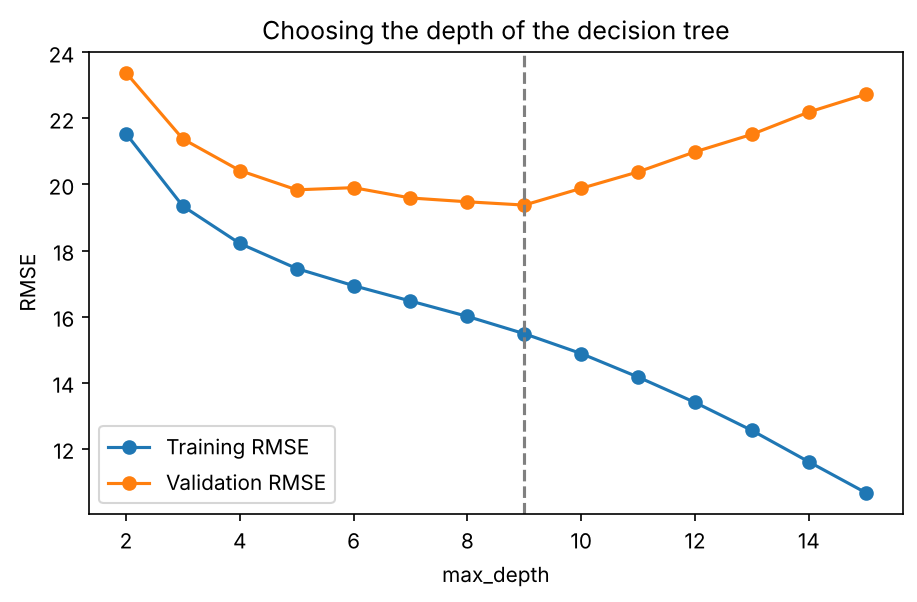
\includegraphics[width=0.95\columnwidth]{depth.png}
\caption{Training and validation RMSE of the decision tree for different depths.}
\label{fig:depth}
\end{figure}

\section{Results}
\begin{table}[t]
\centering\setlength{\tabcolsep}{4pt}
\caption{RUL results on the official test sets (last cycle of each engine, RUL capped at 125).}
\label{tab:res}
\begin{tabular}{lrrrr}
\toprule
& \multicolumn{2}{c}{FD001} & \multicolumn{2}{c}{FD003} \\
Model & RMSE & MAE & RMSE & MAE \\
\midrule
Mean baseline & 43.08 & 34.93 & 42.50 & 35.67 \\
Linear reg. & 21.12 & 17.27 & 21.09 & 16.09 \\
\textbf{Decision tree} & \textbf{18.29} & \textbf{13.09} & \textbf{19.95} & \textbf{13.50} \\
\midrule
CNN~\cite{babu2016} & 18.45 & -- & 19.82 & -- \\
LSTM~\cite{zheng2017} & 16.14 & -- & 16.18 & -- \\
DCNN~\cite{li2018} & 12.61 & -- & 12.64 & -- \\
\bottomrule
\end{tabular}
\end{table}

\begin{table}[t]
\centering
\caption{Logistic regression on all test rows (fail within 30 cycles, threshold 0.5).}
\label{tab:log}
\begin{tabular}{lrr}
\toprule
& Pred.\ OK & Pred.\ fail \\
\midrule
Actually OK & 28,981 & 88 \\
Actually fail & 241 & 382 \\
\midrule
\multicolumn{3}{l}{Accuracy 0.989, precision 0.81, recall 0.61, F1 0.70} \\
\bottomrule
\end{tabular}
\end{table}

The decision tree has the lowest error on both datasets (Table~\ref{tab:res}). On FD001 its RMSE is 58\% lower than the baseline and 13\% lower than linear regression. It is slightly better than the CNN of Babu et al.~\cite{babu2016} on FD001 and about equal on FD003, while the LSTM and deeper CNN are 2 to 7 cycles better.

Logistic regression reaches 98.9\% accuracy (Table~\ref{tab:log}), mainly because only 2\% of test rows are at risk. Its recall of 0.61 means it misses 241 of the 623 at-risk rows.

\begin{figure*}[t]
\centering
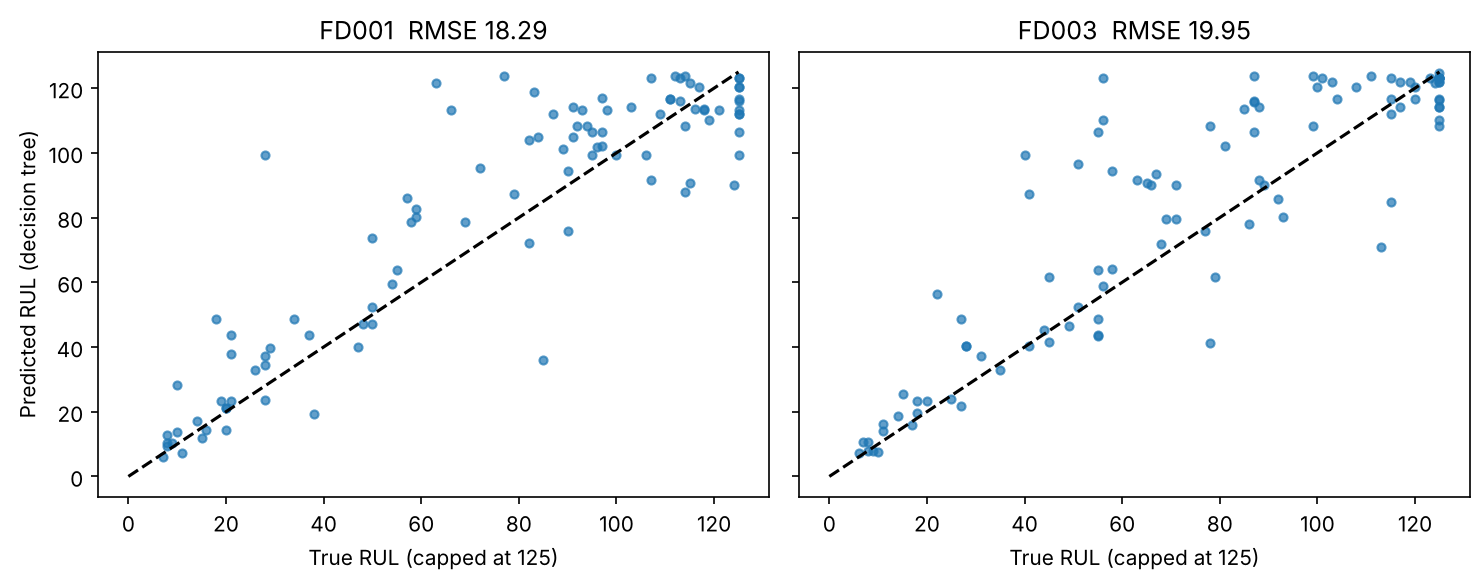
\includegraphics[width=0.7\textwidth]{pred_vs_true.png}
\caption{Predicted vs.\ true RUL of the decision tree for each test engine. The dashed line is a perfect prediction.}
\label{fig:pvt}
\end{figure*}

\begin{figure}[t]
\centering
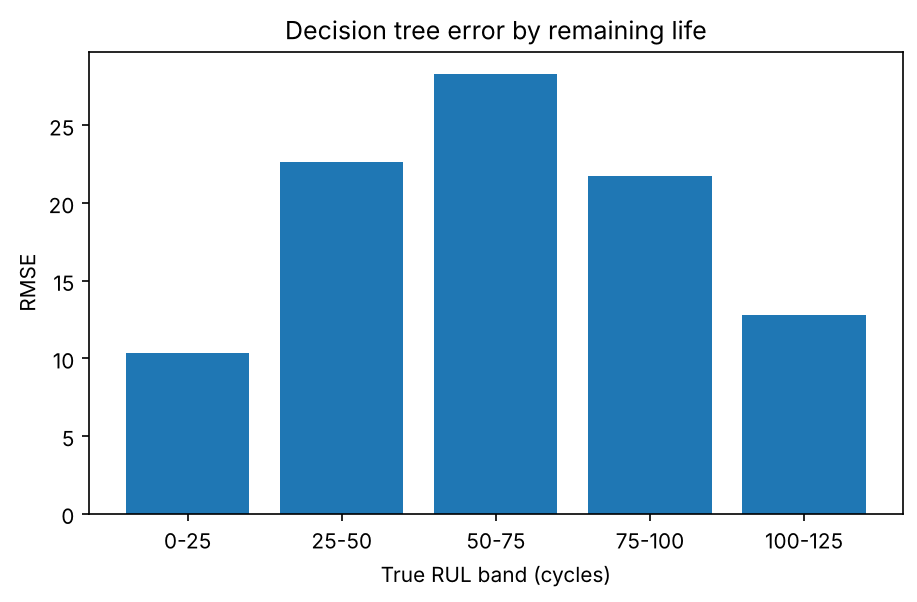
\includegraphics[width=0.9\columnwidth]{error_band.png}
\caption{Decision tree RMSE grouped by true remaining life.}
\label{fig:band}
\end{figure}

\section{Analysis and Discussion}
Near failure the tree is accurate: for engines with fewer than 25 cycles left the RMSE is 10.4 (Fig.~\ref{fig:band}), and most of those points sit on the diagonal in Fig.~\ref{fig:pvt}.

The error is largest for engines with 50 to 75 cycles left (RMSE 28.3), where the average error is $+20$ cycles, so the model thinks these engines are healthier than they are. Of the 200 test engines, 110 are predicted within 10 cycles, 67 are more than 10 cycles late and 23 more than 10 cycles early. The worst, engine FD001\_18, has 28 cycles left but was predicted at 99. In mid-life the wear is still small next to sensor noise, so these engines look new.

FD003 is harder (19.95 against 18.29) because its two faults move some sensors in opposite directions and one model has to learn both patterns.

Some linear regression weights have the opposite sign to their correlation with RUL (s15, for example) because the chosen sensors are correlated with each other (multicollinearity).

The data is simulated with one operating condition, so results may not hold for real engines or FD002 and FD004. We also used one train/validation split and an untuned 0.5 threshold.

\section{Ethical and Legal Considerations}
C-MAPSS is public, simulated NASA data with no personal information, so GDPR does not apply. NASA lists no specific licence and asks users to cite Saxena et al.~\cite{saxena2008,nasadata}. The main risk is safety: a late prediction could delay maintenance on a real aircraft. Such a model should only support engineers and would need testing on real fleet data first.

\section{Conclusion and Future Work}
A decision tree on ten smoothed sensors predicts RUL with RMSE 18.29 on FD001 and 19.95 on FD003, less than half the baseline error and close to an early deep learning model. Logistic regression catches 61\% of at-risk rows. Errors are largest for mid-life engines and when two faults are mixed. Next steps: lower the classification threshold, train one model per fault, try random forests, and test on FD002 and FD004.

\small
\begin{thebibliography}{9}
\setlength{\itemsep}{0pt}
\bibitem{saxena2008} A. Saxena, K. Goebel, D. Simon and N. Eklund, ``Damage propagation modeling for aircraft engine run-to-failure simulation,'' in \emph{Proc. Int. Conf. Prognostics and Health Management (PHM08)}, Denver, CO, 2008.
\bibitem{heimes2008} F. O. Heimes, ``Recurrent neural networks for remaining useful life estimation,'' in \emph{Proc. Int. Conf. Prognostics and Health Management}, 2008, pp. 1--6, doi: 10.1109/PHM.2008.4711422.
\bibitem{babu2016} G. S. Babu, P. Zhao and X.-L. Li, ``Deep convolutional neural network based regression approach for estimation of remaining useful life,'' in \emph{Database Systems for Advanced Applications (DASFAA)}, LNCS 9642, Springer, 2016, pp. 214--228, doi: 10.1007/978-3-319-32025-0\_14.
\bibitem{zheng2017} S. Zheng, K. Ristovski, A. Farahat and C. Gupta, ``Long short-term memory network for remaining useful life estimation,'' in \emph{Proc. IEEE Int. Conf. Prognostics and Health Management (ICPHM)}, 2017, pp. 88--95.
\bibitem{li2018} X. Li, Q. Ding and J.-Q. Sun, ``Remaining useful life estimation in prognostics using deep convolution neural networks,'' \emph{Reliability Engineering \& System Safety}, vol. 172, pp. 1--11, 2018, doi: 10.1016/j.ress.2017.11.021.
\bibitem{nasadata} NASA Prognostics Center of Excellence, ``CMAPSS Jet Engine Simulated Data,'' NASA Open Data Portal. [Online]. Available: \url{https://data.nasa.gov/dataset/cmapss-jet-engine-simulated-data} (accessed 25 Nov. 2026).
\bibitem{sklearn} F. Pedregosa \emph{et al.}, ``Scikit-learn: Machine learning in Python,'' \emph{J. Machine Learning Research}, vol. 12, pp. 2825--2830, 2011.
\end{thebibliography}

\end{document}
